\documentclass[12pt,a4paper]{ctexart}
\usepackage[margin=2.2cm]{geometry}
\usepackage{graphicx}
\usepackage{booktabs}
\usepackage{amsmath}
\usepackage{float}
\usepackage{hyperref}
\usepackage{xcolor}
\usepackage{listings}

\lstset{
  language=Python,
  basicstyle=\ttfamily\small,
  keywordstyle=\color{blue!70!black},
  commentstyle=\color{green!40!black},
  stringstyle=\color{orange!60!black},
  showstringspaces=false,
  breaklines=true,
  frame=single,
  tabsize=4
}

\title{基于 SQuAD 的 Transformer 自动问答实验报告}
\author{姓名：\underline{\hspace{3cm}} \quad 学号：\underline{\hspace{3cm}}}
\date{\today}

\begin{document}
\maketitle

\section{实验目的}
本实验围绕 SQuAD 阅读理解数据集，使用两种基于 Transformer 的问答建模方式完成自动问答任务，目标如下：
\begin{itemize}
  \item 完成基于 Transformer Encoder 的答案区间预测（start/end）任务。
  \item 完成基于 Encoder-Decoder 的序列到序列问答生成任务。
  \item 在示例代码基础上调节关键训练参数（学习率、batch 大小、训练轮次、并行加载参数等），观察其对训练与测试结果的影响。
\end{itemize}

\section{实验过程}
\subsection{实验环境}
\begin{itemize}
  \item 操作系统：Linux
  \item 编程语言：Python 3
  \item 深度学习框架：PyTorch
  \item 关键依赖：transformers、tqdm
  \item 结果输出目录：\texttt{model/}、\texttt{result/}
\end{itemize}

\subsection{数据集与预处理}
\begin{itemize}
  \item 数据集：SQuAD v2.0（\texttt{SQuAD-train-v2.0.json} 与 \texttt{SQuAD-dev-v2.0.json}）。
  \item 输入形式：\texttt{[CLS] question [SEP] context [SEP]}。
  \item 任务一标签：答案起止位置索引（start\_pos, end\_pos）。
  \item 任务二标签：答案文本序列 \texttt{[CLS] answer [SEP]}。
  \item 分词方式：BERT tokenizer（\texttt{bert-base-uncased}），最大长度 256 或 384。
\end{itemize}

\subsection{实现步骤}
\begin{enumerate}
  \item 阅读并保留教师给出的 \texttt{original\_transformerQA1.py} 与 \texttt{original\_transformerQA2.py} 作为基线。
  \item 在 \texttt{transformerQA1.py} 中完成速度与训练稳定性优化（AMP、DataLoader 并行、batch-first 编码器等），并训练 3 个 epoch 保存模型。
  \item 在 \texttt{transformerQA2.py} 中修正自定义 Encoder-Decoder 的掩码与张量维度流，完成训练与测试。
  \item 对两个任务分别执行测试，记录指标并生成结果截图。
\end{enumerate}

\section{实验内容}
\subsection{任务一：Transformer Encoder 区间抽取问答}
该任务把问答建模为答案起点和终点的分类问题。模型输出序列每个位置的起点/终点 logits：
\begin{equation}
\mathcal{L}=\text{CE}(\hat{y}_{start}, y_{start}) + \text{CE}(\hat{y}_{end}, y_{end})
\end{equation}

主要参数：
\begin{itemize}
  \item 批量大小：8
  \item 学习率：$3\times10^{-5}$
  \item 训练轮次：3
  \item 最大序列长度：384
  \item 模型主干：\texttt{nn.TransformerEncoder}（$d_{model}=768$, $nhead=12$, $num\_layers=7$）
\end{itemize}

相对基线代码的主要改动：
\begin{itemize}
  \item 启用混合精度训练（\texttt{autocast + GradScaler}）减少显存占用并提升吞吐。
  \item 将编码器改为 \texttt{batch\_first=True}，减少频繁转置开销。
  \item 增加 DataLoader 并行参数（\texttt{num\_workers/pin\_memory/prefetch\_factor/persistent\_workers}）。
  \item 增加 \texttt{non\_blocking} 数据传输、\texttt{torch.inference\_mode()} 与可选 \texttt{torch.compile}。
\end{itemize}

\subsection{任务二：自定义 Encoder-Decoder 生成式问答}
该任务将问题与上下文编码后，由解码器自回归生成答案序列，损失为词表级交叉熵：
\begin{equation}
\mathcal{L}=\sum_{t=1}^{T} \text{CE}(\hat{y}_t, y_t)
\end{equation}

主要参数：
\begin{itemize}
  \item 批量大小：8
  \item 学习率：$3\times10^{-5}$
  \item 训练轮次：3
  \item 最大序列长度：256
  \item 模型主干：自实现 \texttt{TransformerEncoder/TransformerDecoder}（来自 \texttt{transformerRaw.py}）
\end{itemize}

相对基线代码的主要改动：
\begin{itemize}
  \item 统一张量布局为 batch-first，移除训练/评估阶段不必要的转置。
  \item 修正解码器调用时的掩码传递，显式传入 memory mask。
  \item 完善 \texttt{generate\_answer} 的推理流程（embedding、位置编码、掩码、自回归终止条件）。
\end{itemize}

\section{实验结果}
\subsection{任务一结果：三轮模型测试对比}
\begin{figure}[H]
\centering
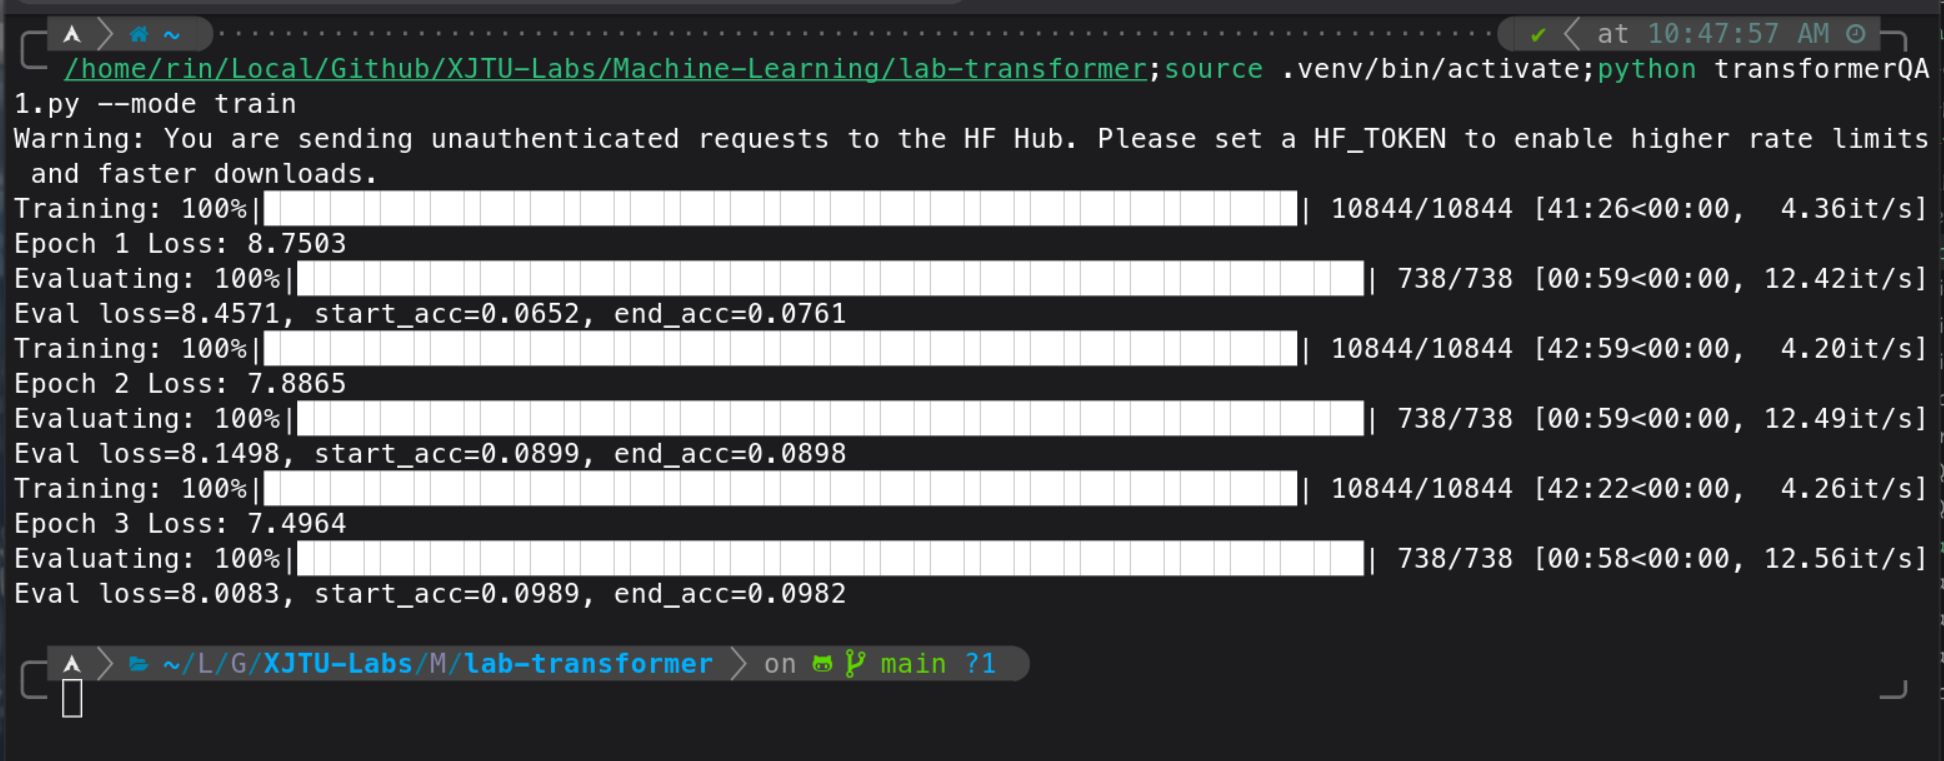
\includegraphics[width=0.95\textwidth]{images/QA1_running_result.png}
\caption{任务一训练过程与评估日志截图}
\label{fig:qa1_train_log}
\end{figure}

\begin{figure}[H]
\centering
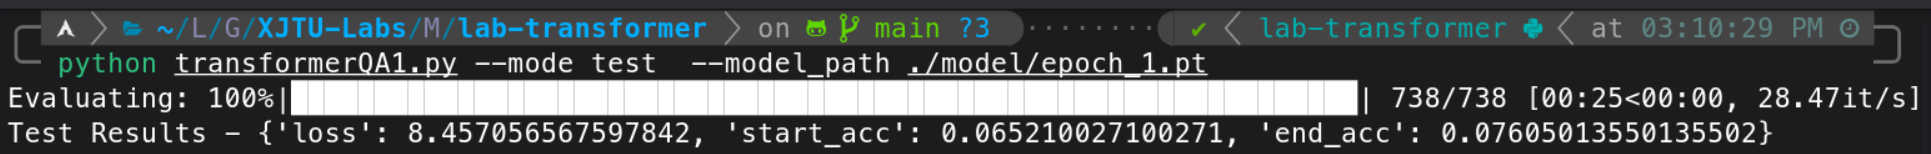
\includegraphics[width=0.31\textwidth]{images/QA1_epoch1_test_result.png}
\hfill
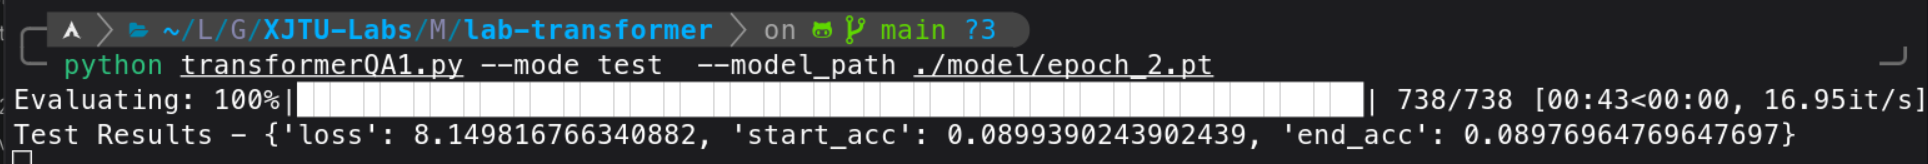
\includegraphics[width=0.31\textwidth]{images/QA1_epoch2_test_result.png}
\hfill
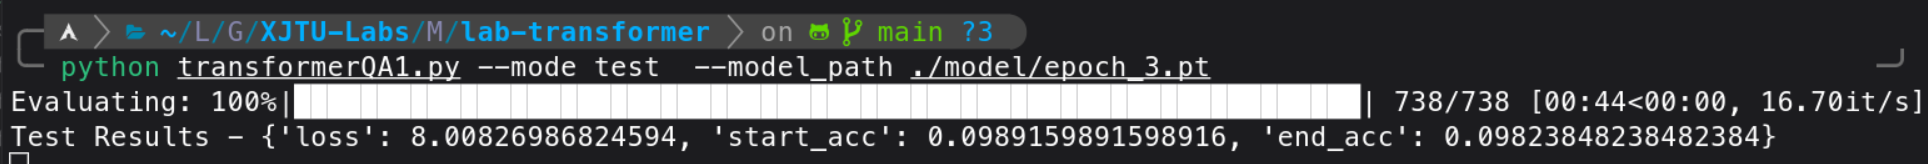
\includegraphics[width=0.31\textwidth]{images/QA1_epoch3_test_result.png}
\caption{任务一：epoch\_1/2/3 模型在测试模式下的结果截图}
\label{fig:qa1_test_log}
\end{figure}

\begin{table}[H]
\centering
\caption{任务一测试指标（来自三次测试截图）}
\label{tab:qa1_metrics}
\begin{tabular}{lccc}
\toprule
模型 & Test loss & start\_acc & end\_acc \\
\midrule
epoch\_1.pt & 8.4571 & 0.0652 & 0.0761 \\
epoch\_2.pt & 8.1498 & 0.0899 & 0.0898 \\
epoch\_3.pt & 8.0083 & 0.0989 & 0.0982 \\
\bottomrule
\end{tabular}
\end{table}

结果分析：
\begin{itemize}
  \item 随 epoch 增加，测试损失从 8.4571 下降到 8.0083，start/end 准确率持续上升。
  \item 说明 Encoder 抽取式模型已经学习到一定的对齐关系，但绝对精度仍偏低，任务仍有较大优化空间。
  \item 结合训练日志，模型训练损失下降明显快于测试指标提升，存在一定泛化瓶颈。
\end{itemize}

\subsection{任务二结果：Encoder-Decoder 测试损失}
\begin{figure}[H]
\centering
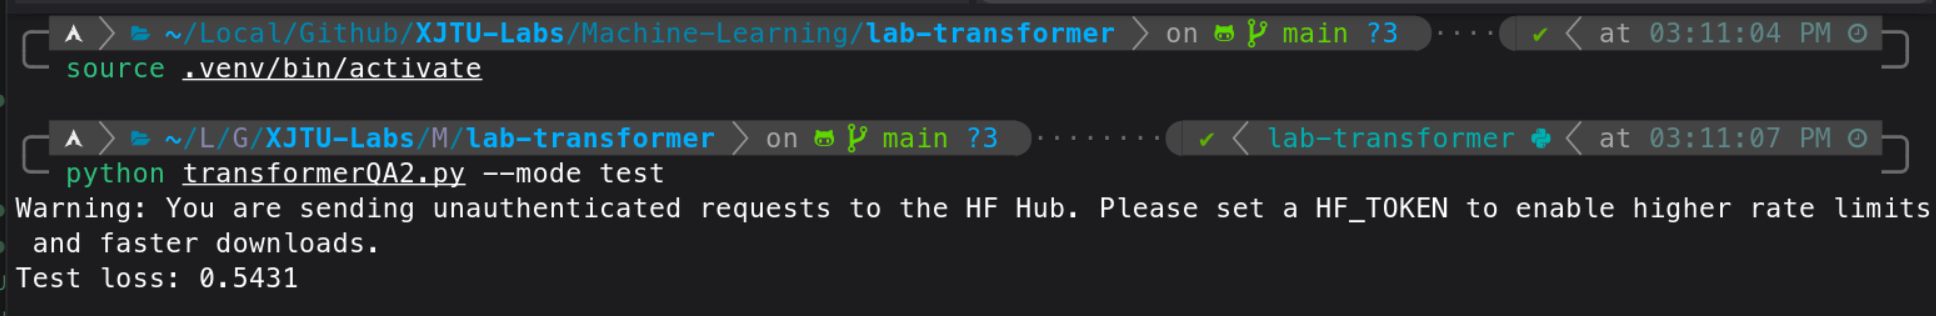
\includegraphics[width=0.95\textwidth]{images/QA2_test_result.png}
\caption{任务二测试结果截图（\texttt{python transformerQA2.py --mode test}）}
\label{fig:qa2_test_log}
\end{figure}

同时根据 \texttt{result/QA2\_running\_result.txt} 的训练日志，3 个 epoch 的指标如下：
\begin{table}[H]
\centering
\caption{任务二训练/验证损失变化}
\label{tab:qa2_metrics}
\begin{tabular}{lcc}
\toprule
Epoch & train\_loss & dev\_loss \\
\midrule
1 & 2.9827 & 1.7377 \\
2 & 1.2329 & 0.8976 \\
3 & 0.6251 & 0.5431 \\
\bottomrule
\end{tabular}
\end{table}

结果分析：
\begin{itemize}
  \item 任务二的损失下降趋势明显且稳定，最终 dev/test loss 约为 0.5431。
  \item 相比任务一，生成式模型在当前配置下给出了更低的 loss 指标。
  \item 但该指标仅衡量 token 级别拟合程度，后续还需引入 EM/F1 或 BLEU 等文本质量指标进行更全面评估。
\end{itemize}

\section{总结}
本实验完成了 SQuAD 自动问答任务中的两类 Transformer 建模：
\begin{itemize}
  \item 完成了基于 Transformer Encoder 的抽取式问答训练与多轮测试，验证了模型随训练轮次的收敛趋势。
  \item 完成了基于自定义 Encoder-Decoder 的生成式问答训练与测试，获得了更低的验证损失。
  \item 在示例代码基础上实现了关键工程改进（AMP、并行数据加载、掩码修正、维度流修正），提高了代码可运行性与训练效率。
\end{itemize}

后续可继续从模型规模、学习率调度、答案后处理与评价指标扩展（EM/F1）等方向优化结果。

\section*{附录：实验源代码与运行命令}
\subsection*{A.1 主要修改点代码片段（transformerQA1.py / transformerQA2.py）}
\begin{lstlisting}
# QA1: mixed precision + batch_first encoder + dataloader optimization
with autocast("cuda", enabled=(self.config.use_amp and self.config.device.type == "cuda")):
    s_logits, e_logits = self.model(input_ids, mask)
    loss = self.criterion(s_logits, start) + self.criterion(e_logits, end)

encoder_layer = nn.TransformerEncoderLayer(
    d_model=config.d_model,
    nhead=config.nhead,
    dim_feedforward=config.dim_feedforward,
    dropout=config.dropout,
    batch_first=True,
)

# QA2: keep batch-first, pass memory mask explicitly
outputs = self.model(src, decoder_in, src_mask, tgt_mask)

output = self.decoder(tgt, memory, tgt_mask, src_mask)
\end{lstlisting}

\subsection*{A.2 运行命令}
\begin{verbatim}
# 任务一训练
python transformerQA1.py --mode train

# 任务一测试（分别测试三个 epoch）
python transformerQA1.py --mode test --model_path ./model/epoch_1.pt
python transformerQA1.py --mode test --model_path ./model/epoch_2.pt
python transformerQA1.py --mode test --model_path ./model/epoch_3.pt

# 任务二训练与测试
python transformerQA2.py --mode train
python transformerQA2.py --mode test
\end{verbatim}

\end{document}
